\documentclass{scrartcl}
\usepackage[mathletters]{ucs}
\usepackage[utf8x]{inputenc}
\usepackage{amssymb}
\usepackage{amsmath}
\usepackage[usenames]{color}
\usepackage{hyperref}
\usepackage{wasysym}
\usepackage{graphicx}
\usepackage[normalem]{ulem}
\usepackage{enumerate}

\usepackage{listings}

\lstset{ %
basicstyle=\footnotesize,       % the size of the fonts that are used for the code
showspaces=false,               % show spaces adding particular underscores
showstringspaces=false,         % underline spaces within strings
showtabs=false,                 % show tabs within strings adding particular underscores
frame=single,                   % adds a frame around the code
tabsize=2,                      % sets default tabsize to 2 spaces
breaklines=true,                % sets automatic line breaking
breakatwhitespace=false,        % sets if automatic breaks should only happen at whitespace
}


\title{Masterproef Tool Wear Inspection - Update 4 TG}
\date{dinsdag 08 december 2020}
\author{}

\begin{document}

\maketitle

		\section{Masterproef Tool Wear Inspection - Update 4 TG}

Created vrijdag 20 november 2020



\subsection{Mail}

Beste meneer Goedemé,

 

Ik voer de masterproef over Tool Wear Inspection uit bij Eavise in samenwerking met Sirris waarbij de slijtage van freeskop snijplaatjes gemeten moet worden.

Gezien we ongeveer in de helft van de periode tot het tussentijds verslag zitten wilde ik u als promotor graag een korte update geven over de vorderingen die reeds gemaakt zijn en wat er nog staat te gebeuren. Indien u wenst kunnen we ook eens een korte vergadering inplannen of typ ik een verslagje uit zodat ik u volledig op de hoogte kan stellen.

 

In het heel kort heb ik mij tot nu vooral bezig gehouden met het maken van een (semi geautomatiseerde) camera opstelling die per 20 snijplaatjes de nodige beelden kan maken met verschillende belichtingshoeken en verschillende kleuren belichting.

Van de plaatjes zit een foto in bijlage. Deze zijn ongeveer 0,5cm op 1cm en hebben een slijtage die met het oog nauwelijks zichtbaar is. A picture containing building, floor, sitting, table



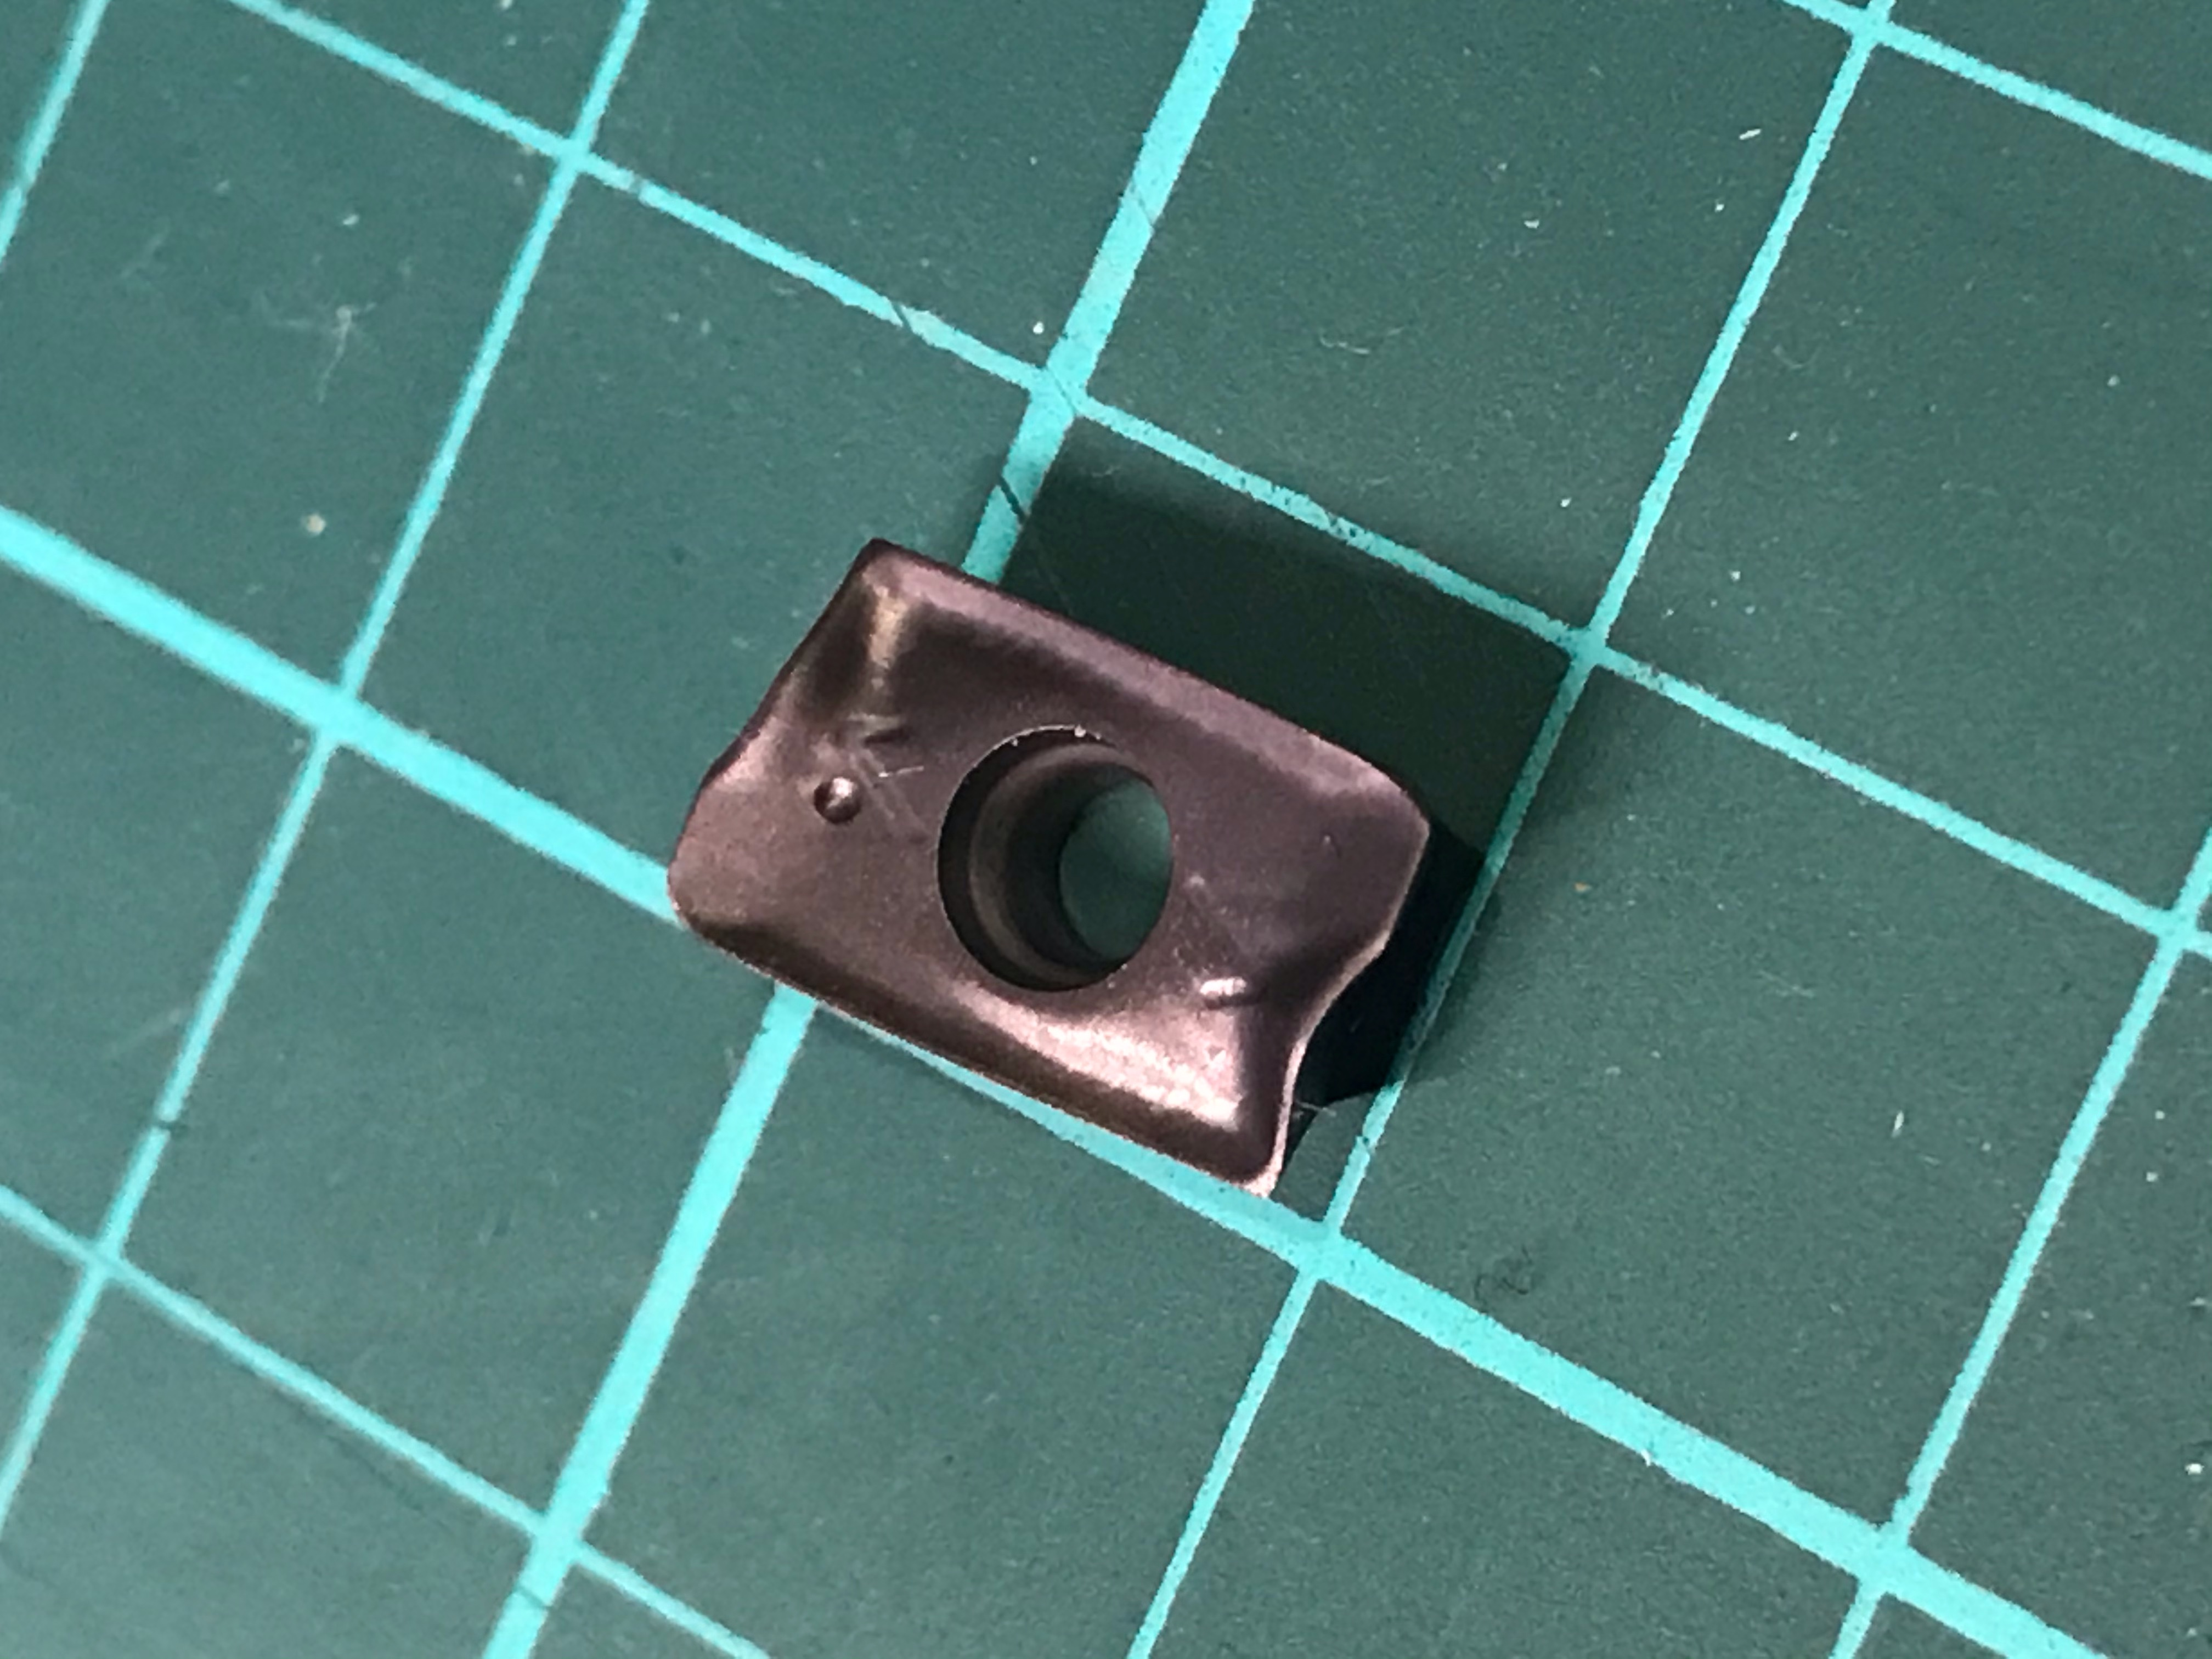
\includegraphics[width=4.166667in, keepaspectratio=true]{./Masterproef_Tool_Wear_Inspection_-_Update_4_TG/plaatje_1cm.jpeg}



Ik heb al een aantal beelden kunnen maken (in bijlage te vinden), maar er is nog wat finetuning nodig om de camera positie en hoek beter te kunnen regelen om ook de invloed daarvan te kunnen meten.

De komende weken zal ik deze opstelling nog afwerken en zoeken naar een ideale camera hoek door wat beelden door een simpel netwerk laten gaan en de resultaten te vergelijken voor verschillende camera posities waarbij de licht condities niet wijzigen.

 

Met vriendelijke groeten,

 

Lars De Pauw



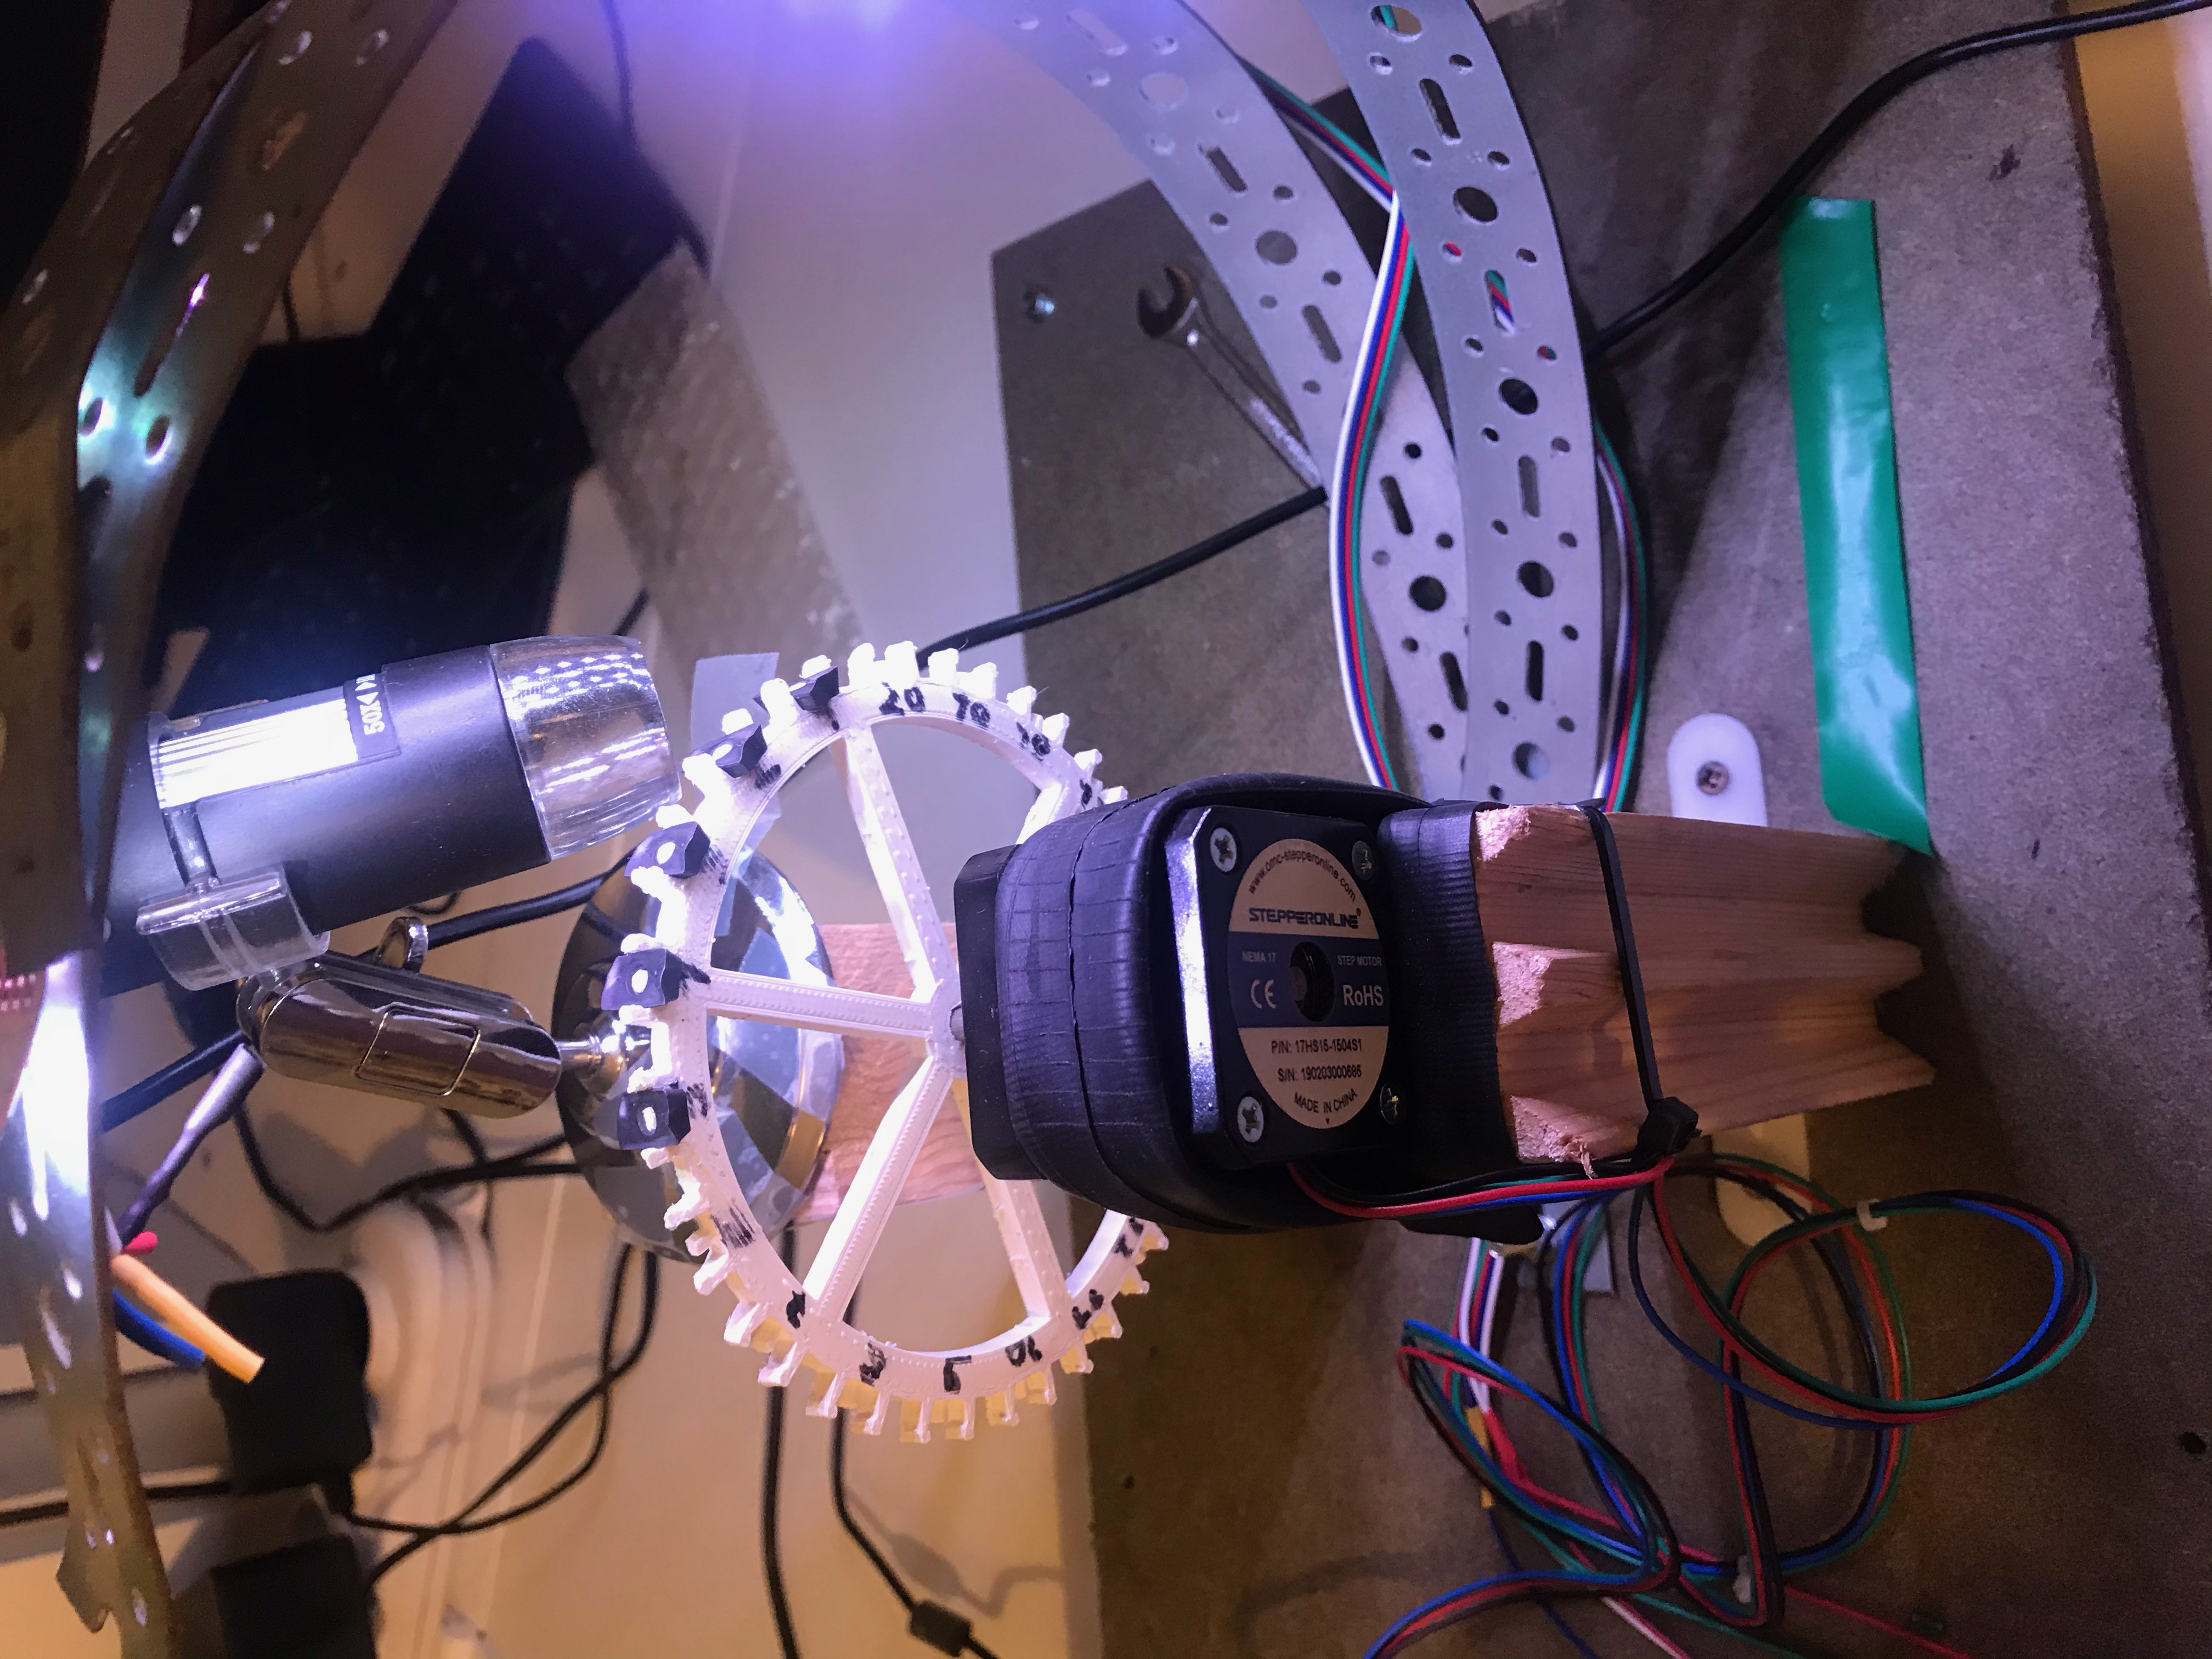
\includegraphics[width=4.166667in, keepaspectratio=true]{./Masterproef_Tool_Wear_Inspection_-_Update_4_TG/rechts_licht.jpeg}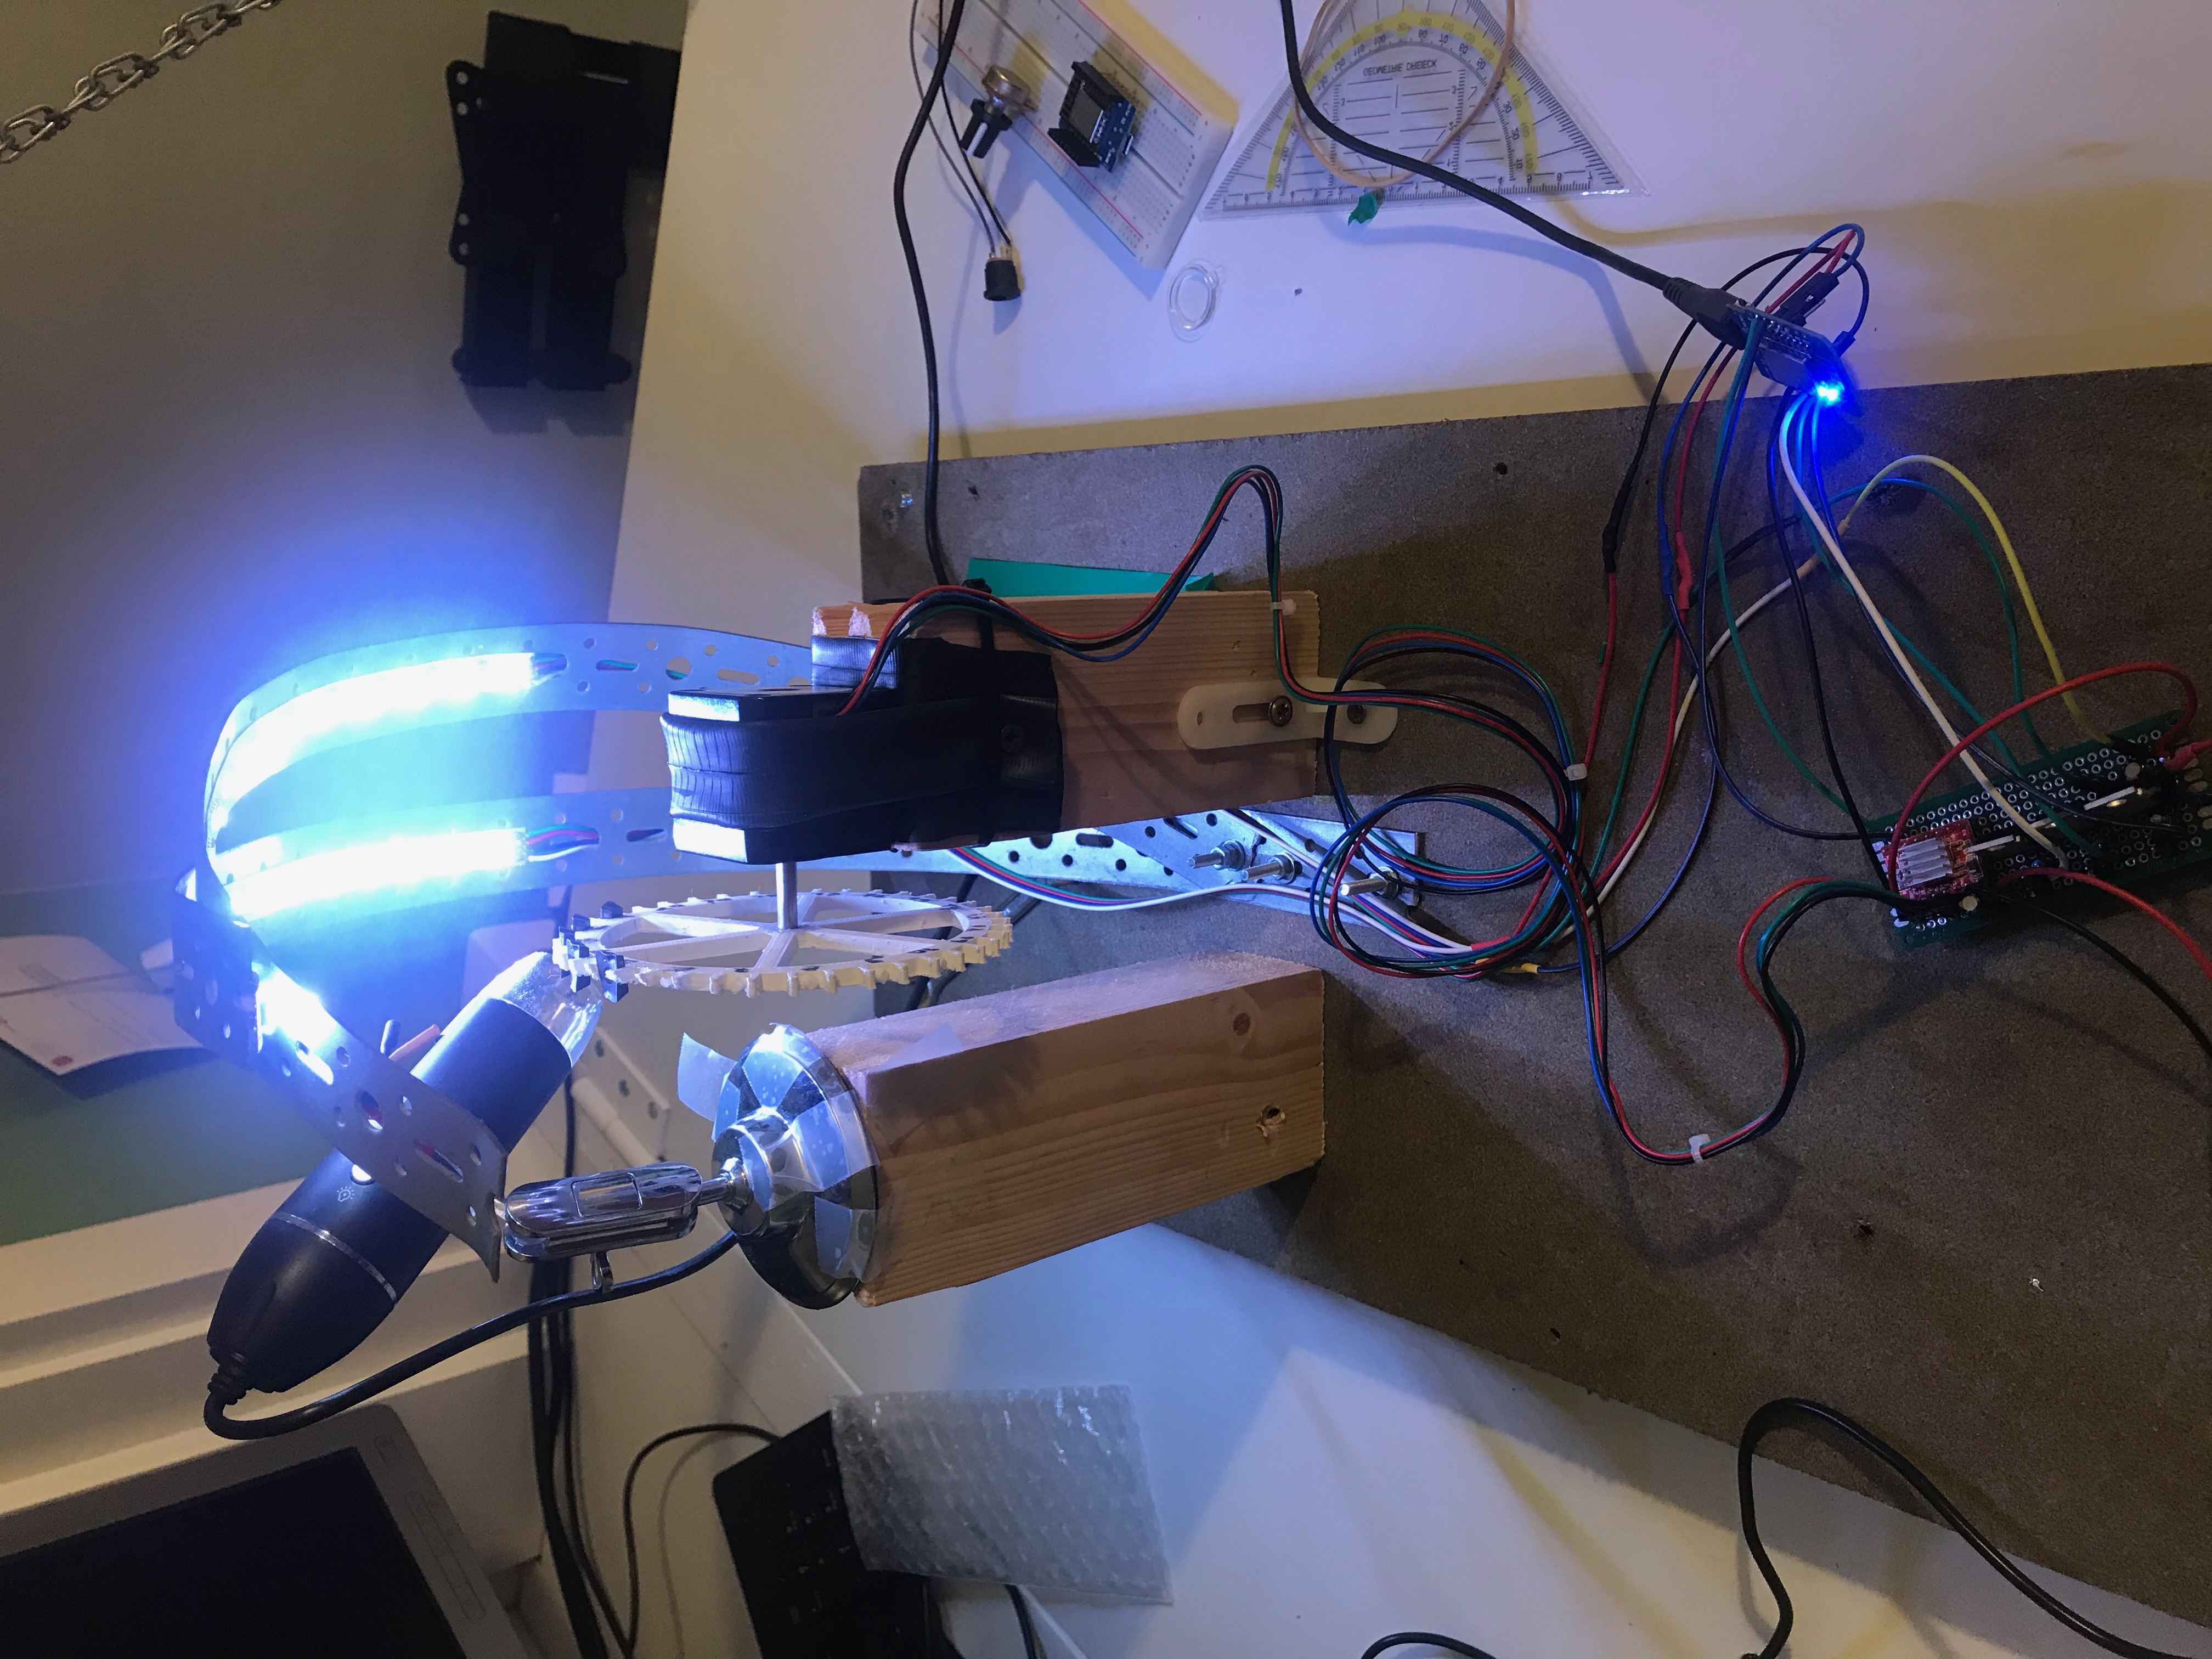
\includegraphics[width=4.166667in, keepaspectratio=true]{./Masterproef_Tool_Wear_Inspection_-_Update_4_TG/achter_licht.jpeg}



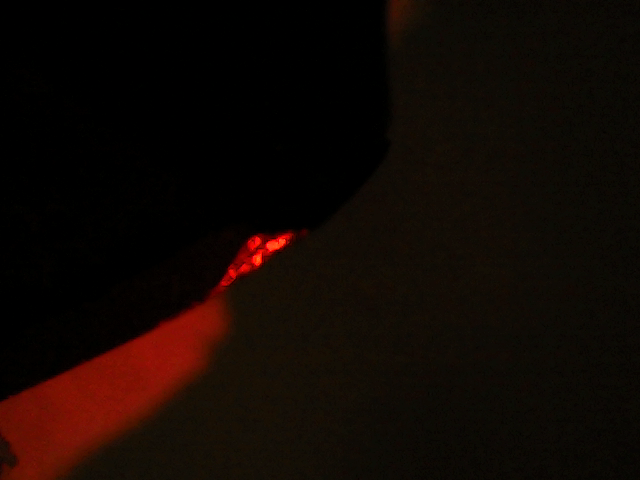
\includegraphics[width=4.166667in, keepaspectratio=true]{./Masterproef_Tool_Wear_Inspection_-_Update_4_TG/p4_l9.png}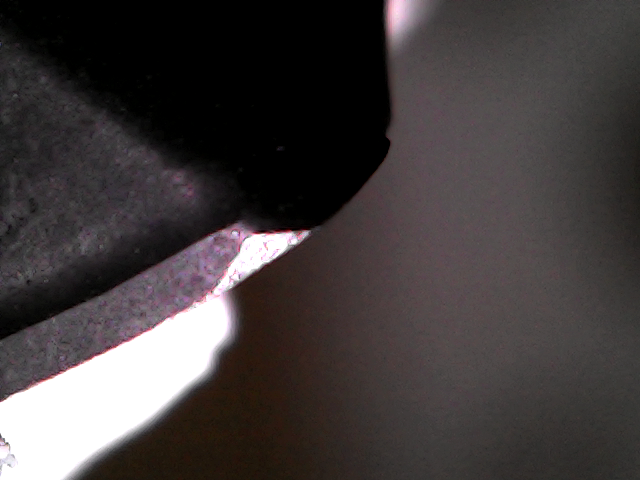
\includegraphics[width=4.166667in, keepaspectratio=true]{./Masterproef_Tool_Wear_Inspection_-_Update_4_TG/p4.png}



\end{document}
